\chapter{Working with the Data Explorer}

\section{Loading data}

\subsection{Data Types}
\label{datatypes}

\ogs distinguishes between different types of data such as geometry, meshes and process-dependent data. The \emph{Data View} of the Data Explorer reflects this distinction by separating all the data loaded into the programme into one of the four tabs of the data view:

\begin{figure}[tb]
\begin{center}
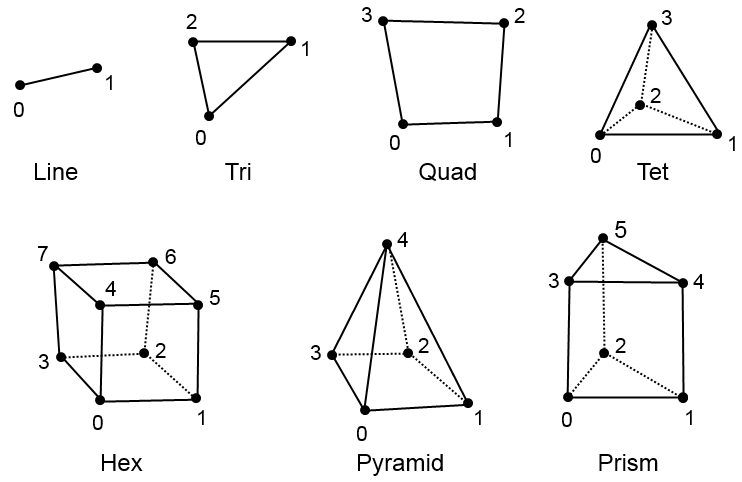
\includegraphics[width=0.95\linewidth]{elementtypes}
\caption{Mesh element types supported by \ogs.}
\label{fig:elements}
\end{center}
\end{figure}

\begin{itemize}
\item \textbf{Geometrical data} includes points, polylines and surfaces. To be more specific, points include any location in 3D space by giving an $x$, $y$ and $z$ coordinate. Lines are a ordered list of points, the can closed to represent polygons by specifying the first and last point of the line to be identical. Finally, surfaces are composed of triangles, which in turn are consisting of three points. To decide which direction a triangle is facing, points are given in counter-clockwise order on the ``up-side''.\index{Geometry}
\item \textbf{Meshes} are domain discretisations in 2D or 3D. Each mesh contains a set of nodes (points) as well as a set of elements defined by a subset of these nodes. A mesh may contain different kinds of elements. OGS supports the following element types\index{Element types}: lines, triangles, quadrilaterals, tetrahedra, hexahedra, pyramids, prisms. See figure \ref{fig:elements} for example elements and node numbering.\\
    Meshes are often classified into structured or unstructured meshes. Note, that \ogs treats all meshes as unstructured, independent of their actual structure.\index{Meshes}
\item \textbf{Stations} include observation sites of data loggers or boreholes. This data differs from geometry as it contains additional information for each object such as stratigraphic information for boreholes or time series data for data loggers. Within the Data Explorer this data is visualised in a different way.\index{Observation Sites}
\item \textbf{Modelling data} supported by the data explorer is currently only a listing of processes with their primary variables as well as initial- and boundary conditions. These conditions can be applied to geometrical objects or mesh nodes and these will also be visualised in the render window.\index{FEM Conditions}
\end{itemize}


\subsection{Native File Formats}
\label{nativefileformats}
\index{File formats}

\ogs has a large number of native file formats for storing geometrical data, meshes, processes, FEM conditions (such as boundary conditions) and material properties (e.g. fluid properties) and many more.

Not all of them can be loaded into the user interface since not all of them contain data that can be visualised. Things are additionally made difficult as the file standards for the programm are currently changed from GeoSys4 legacy files in ASCII format to XML files\footnote{http://www.w3.org/XML/}. For this reason there exists -- at least at the time of this writing -- two file standards for certain kinds of data. Hopefully, this unfortunate situation is resolved soon.

You can open native OGS files by clicking \cmd{File\ra Open...}\index{Loading geometry}\index{Loading meshes} or by clicking the folder icon in the respective Data View tab. Please note that the file \emph{must} have the correct file extension for the programme to correctly recognise the type.

Supported XML file formats are:
\begin{itemize}
\item Geometry files: *.gml\\
        Points, polylines and surfaces\index{Geometry}
\item Meshes: *.vtu\index{Meshes}\\
        Domain discretisations. Note that this is a VTK-file format and you can use these exact files also in other VTK compliant software such as ParaView\index{ParaView}.
\item Observation sites: *.stn\\
        Boreholes and data logger sites.\index{Observation Sites}
\item FEM Conditions: *.cnd\\
        Boundary conditions, initial conditions and source terms needed for simulation of processes. These files contain information that links phenomena with a given set of values (or distribution of values) to geometric objects or mesh nodes.\index{FEM Conditions}
\item \ogs project files: *.gsp\index{Project files}\\
    These files contain file-paths related to a given project. All of files listed within will be loaded upon loading the *.gsp file. This is especially useful for projects consisting of a large number of input files.
\end{itemize}

Legacy files that are still supported for the time being:
\begin{itemize}
\item Geometry: *.gli
\item Meshes: *.msh
\item FEM Conditions: *.bc, *.ic, *.st
\end{itemize}


\subsubsection{Additional Information about Loading FEM Conditions}
\index{Loading FEM conditions}

Besides loading FEM Conditions via  \cmd{File\ra Open...}, it is also possible to right-click on any geometry in the data view to assign FEM conditions to a geometry via \cmd{Load FEM Condition...}. Upon loading it is checked if a corresponding geometry for these conditions is available. For XML-files the associated geometry name is saved in the cnd-file, for old file types it is simply assumed that the geometry name will be the same as the name of the condition-file. If no geometry of this name is found, the data will not be loaded. You may may also add source terms of the process distribution ``DIRECT'' directly on meshes nodes (again, via right-clicking on a mesh) and the conditions will then be displayed on the respective mesh nodes defined in the input file.

For the visualisation, the correct scalar values in the render window will currently only be displayed for process distribution types ``CONSTANT'', ``LINEAR'' and ``DIRECT''.\footnote{For an overview over what process distribution types are, which types are supported by the system and how they influence a subsequent simulation please refer to a technical documentation of \ogs.}

\subsubsection{Conversion of Native Files}
\index{OGS File Converter}

It is possible to convert data between GeoSys4 ASCII files and \ogs XML files (and vice versa) via the \emph{OpenGeoSys File Converter}. The file converter can be called from \cmd{Tools\ra File Converter...} and is also available as a stand-alone tool upon download of \ogs. Simply select which type of file you would like to convert, specify file names and press okay.

The file converter currently supports conversion of geometry and FEM condition files, but will be extended in the future as file formats are changed to XML.

\subsection{Import File Formats}
\label{Import File Formats}
\index{Import file formats}

\begin{figure}[tb]
\begin{center}
\includegraphics[width=0.99\linewidth]{interfaces}
\caption{Supported file formats for import and export of data.}
\label{fig:interfaces}
\end{center}
\end{figure}

A number of non-native file formats can also be loaded and visualised in the Data Explorer. To import these files click on \cmd{File \ra Import Files} and select the appropriate entry.

Depending of which file format you want to load, quality of the interface varies depending on a number of facts such as if the file format is an open standard or if there were enough input files to test the interface when it was implemented.

Currently the following file formats are supported:
\begin{itemize}
\item ESRI \textbf{shape} files (*.shp)\index{Shape files}\\
Vector files specifying points, polylines and polygons. The interface for shape files is thoroughly tested and there should be no problems whatsoever. However, note that a lot shape files come with a database file containing additional information (*.dbf) which has no standardised table structure and therefore is not analysed or imported by the data explorer.
\item Aquaveo \textbf{GMS} files (*.txt, *.3dm)\index{GMS files}\\
Text or mesh files specifying boreholes (*.txt) or layered meshes build from tetrahedrons and prisms. This interface has been tested with number of cases and should work fine.
\item \textbf{GMSH} files (*.msh)\index{GMSH files}\\
Mesh files containing unstructured grids. As an exception these files are \emph{not} loaded via the import menu but you have to load them directly via \cmd{File\ra Open...}. The interface should work perfectly however.
%\item \textbf{GoCAD} files (*.ts)\index{GoCAD files}\\
%This interface is in an unfinished state. However, there exists a programming interface to write OGS-files directly from GoCAD. Please talk to the development team if you need to load data into OGS.
\item \textbf{NetCDF} files (*.nc, *.cdf)\index{NetCDF files}\\
A machine-independent format that contains all kinds array-oriented scientific data. The interface only works from GUI as it requires to open a dialogue where data dimensions and time steps need to specified. The netCDF date will then be converted into either a mesh or a raster. Conversion into a mesh allows to set more parameters such as the requested mesh element type and the data representation (also see section \ref{meshraster}).
\item \textbf{FEFLOW} files\index{FEFLOW files}\\
Allows the import FEFLOW problem ASCII files (*.fem). This interface imports only geometry, e.g. polygons, and meshes.
\item \textbf{Petrel} files\index{Petrel files}\\
This interface is in an unfinished state. Please talk to the development team if you need to load data into OGS.
\item \textbf{Raster} files (*.asc, *.bmp, *.jpg, *.grd *.png, *.tif)\index{Raster files}\index{Images}\\
Image data files that may contain satellite images, etc. ESRI and Surfer ASCII raster files (*.asc / *.grd) as well as GeoTIFF (*.tif) files contain geo-referenced data, while common image files (*.bmp, *.jpg, *.png) do not. This interface should work for all supported file types although it can be quite slow for large raster files.
\item \textbf{TetGen} files\index{TetGen files}\\
Allows the import files created with the TetGen mesh generator. This interface currently only reads the node- and tetrahedra-files created by the software (i.e. *.node and *.ele).
\item Visual Toolkit (\textbf{VTK}) files (*.vti, *.vtk, *.vtp, *.vtr, *.vts, *.vtu)\index{VTK files}\\
Files containing data for graphic objects, ranging from image files (*.vti) to structured (*.vts) or unstructured meshes (*.vtu). All data sets may include additional data in the form of scalar arrays. This interface should work perfectly.
\end{itemize}

\begin{figure}[tb]
\parbox[b]{.45\linewidth}{
    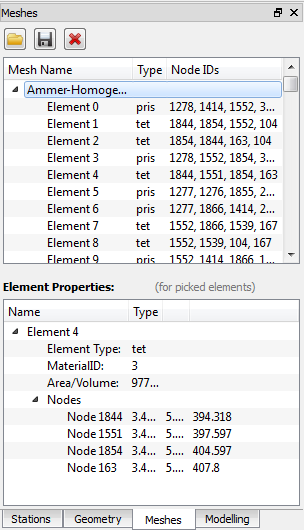
\includegraphics[width=.95\linewidth]{dataview}
}
\parbox[b]{.55\linewidth}{
    \caption{The \emph{Data View} offers detailed information on loaded data sets. The icons on top will provide general functionality for this tab: The folder icon allows to open files, the disc icon is for saving data sets and the cross icon will remove the selected data set. The tabs at the bottom of the Data View will open the views for the respective kind of data. Right-clicking data sets will give options for additional, data-set related functionality.\\
    The Mesh View depicted to the left also includes an additional window for viewing mesh element properties. This window will only contain information upon selecting a mesh element in the Data View above or in the Render Window.}
}
\label{fig:interfaces}
\end{figure}

\subsection{Saving Data}
\index{Saving data}

\section{Writing Data}
\index{Saving data}

\subsection{Native Files}

The \ogs Data Explorer offers functionality to modify data sets loaded into the programme. Details will be given in the following sections but examples include the concatenation of polylines, merging material groups in meshes or creating new boundary conditions on geometric objects.

To save this newly created or modified data, select the data set in its respective Data View and click the disc icon on top of the tab. A dialog to save the file will open and a location and filename for the data can be chosen.

You can also save all loaded data files by saving an \ogs project. Select \cmd{File\ra Save as...} and specify a project name. This option will save all geometries in *.gml files, all mesh meshes in *.msh files and all observation sites in *.stn files. Additionally it will create a project file (*.gsp). When loading the gsp-file later on it will also load the respective geometries and observation sites again. (Note: Other file formats -- e.g. for boundary conditions or processes -- will be added in the future)

\subsection{Export to Other Formats}
\index{Export formats}

Any geometric data loaded into \ogs can be exported into a GMSH *.geo file via \cmd{File\ra Save as...} and selecting ``GMSH gemetry files'' as the output format. Note, that this will merge all geometries loaded into the programme and that it will also save station-data as points (i.e. you lose any additional information associated with these stations). Before saving, the geometric information will be inserted into a quad tree structure to analyse the data and insert additional points (so-called `Steiner Points') at locations where not enough information for generation of a suitable mesh exists. This ensures the creation of an adequate result when meshing the geo-file within GMSH.\footnote{Note that this allows you to export any combination of data into GMSH format for subsequent meshing. The functionality described in section \ref{meshcreation} for meshing of data within \ogs requires a ``bounding polygon'' that serves as outer boundary of all the data contained within the mesh.}

\bigskip

You can also export data from \ogs into a number of graphics formats. This can be done for selected graphical objects by right-clicking the respective object in the visualisation pipeline and than select the desired format (VTK, Unity3D or OpenSG). Details on this can be found in section \ref{specvisoptions}.

You can also export the complete scene into the graphic formats VTK, OpenSG or VRML format. To do this select \cmd{File\ra Export\ra Format}.

\section{Removing Data}
\index{Removing data}

You can remove a data set loaded into \ogs by selecting the data set in its respective Data View and then pressing the red cross icon on top. Specifically you can also remove only polylines or surfaces only from a geometry. The only exception to this rule are geometric points which can only be removed if both surfaces and polylines are already deleted as both kinds of objects are dependent on points. Regardless of the previous remarks you can also remove geometries as whole.

\section{Data Visualisation}
\label{datavisualisation}

Technically, data (or a representation thereof) loaded into the programme is displayed at three different locations in the Data Explorer (see figure \ref{fig:gui}):

\subsection{Data Views}
\index{DataView}

There are four different DataView-Tabs in the programme where the data is visible in the form of lists. Which of the tabs is used depends on the data. There is one tab for geometrical information, one for meshes, one for stations (i.e. observation sites) and one for modelling information (i.e. processes, boundary conditions, etc.)

The DataView for geometrical information contains a list of geometries. Each geometry-item has up to three children titled ``Points'', ``Polylines'' and ``Surfaces'' containing the information about the respective geometrical objects. For example, the item `Points' contains a list of points and for each item (i.e. each point) its index, the coordinates and (if existing) the name of the object can be displayed. Each geometry \emph{needs} to contain a list of points. Other geometrical objects (i.e. polylines or surfaces) are optional. Upon selecting a geometrical object in the DataView, the object will also be highlighted\index{Highlighting objects} in the render window. For better visibility a point will be marked by a small ball and a line by a tube.

Note, that the mesh-tab is subdivided into a view of the meshes loaded into the programme (and the elements contained within each mesh) and a second window called ``Element Properties''. If an element is selected in the Data View or picked from the Render Window, all available information concerning that element (such as nodes, volume, element type, etc.) will be displayed here. Likewise, if an element is selected in Data View it will be highlighted in the Render Window. As the element information becomes available under Element Properties, it is also possible to select a node from nodes list of the selected element. This node will then be highlighted as a small ball in the Render Window, similar to geometric points.

\subsection{Render Window}
\index{Render window}

\begin{figure}[tb]
\begin{center}
\subfloat{\includegraphics[width=0.48\linewidth]{error1}}\enspace
\subfloat{\includegraphics[width=0.48\linewidth]{error2}}
\end{center}
\caption{Examples for inconsistencies within the data. The left image show inconsistencies between two meshes. The right images show a number of boreholes, one of which has a wrong offset.} \label{fig:error}
\end{figure}

The render window is the part of the GUI where all the data is visualised in a user-controlled 3D scene. The process of ``drawing'' an object in the render window is technically called the \emph{rendering} of the object and will be referred to as such in the following. The Render Window is where the data is actually displayed and where all the effects of changes done in other parts of the programme or to the input data will be visible.

One of the big advantages of the Data Explorer is in the fact that this visual inspection of the data also allows you to assess your data and to find inconsistencies and errors. Figure \ref{fig:error} gives examples of such inconsistencies.

The 3D view can be manipulated using the mouse. Holding the left mouse button and moving the mouse will rotate\index{Rotating} everything around the focal point of the scene. By default this is the center point of all data loaded into the programme. By holding the middle mouse button it is possible to pan the view, resulting in a translation\index{Translation} left / right and up / down. By holding the right mouse button or moving the mouse wheel the complete scene will be zoomed\index{Zooming} in and out.

There is an alternative mouse button functionality assignment which is activated by holding the Spacebar. When activated, left clicks pick\index{Picking} a cell of the actually selected visualisation pipeline object. This allows to mark a certain cell of the visualisation, such as a mesh element for displaying information related to that element in Element Properties is detailed in the previous section. On right-clicking, the picked position is set as the new focal point of the camera\index{Focal Point}. This is useful for a better examination of an interesting region of the data so with focal point set to that region you can easily rotate and zoom around.

The selected cell can be de-selected again by holding Spacebar and clicking somewhere into the background of the render window.

\subsection{Render Window Options}

\begin{figure}[tb]
\begin{center}
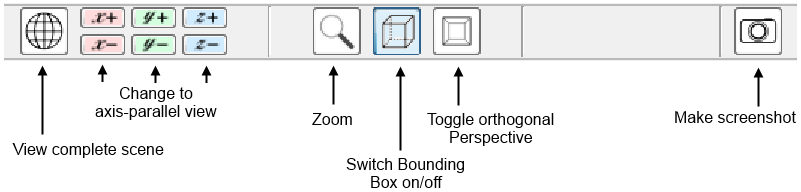
\includegraphics[width=0.8\linewidth]{renderwindowoptions}
\caption{Available options for the Render Window}
\label{fig:renderoptions}
\end{center}
\end{figure}

A button bar is located right above the Render Window where some general options concerning the current scene can be set (see figure \ref{fig:renderoptions}). A set of six buttons on the left site allows axis-parallel viewing the scene from both ends of the three coordinate axes \index{Axis-parallel view}. The ``Globe''-icon on the left side gives a view of the complete scene from above and is thus equivalent to the $+z$ icon.

The magnifying glass icon allows to zoom into the scene\index{Zooming}. When this icon is toggled, pressing the left mouse button will no longer rotate the scene but instead draw a frame into which the programme will zoom upon releasing the mouse button. The second button in this group toggles the visualisation of a bounding box\index{Bounding Box} around the object currently selected in the visualisation pipeline. The third button switches between perspective projection and orthogonal projection\index{Projection}.

The right-most button depicting the camera-icon will result in a screenshots\index{Screenshots} of the current content of the render window. Upon pressing the Button a small dialogue will open that allows to select the scaling factor for the saved image. This is useful for creating large image (e.g. for posters) without artefacts.

\subsection{Visualization Pipeline}
\index{Visualization pipeline}

The Visualisation Pipeline looks very similar to the Data Views described in section \ref{datatypes}. However, the items displayed in this tab are a list of the graphical objects displayed (rendered) in the Render Window. For further reference these will be called \emph{pipeline items}. Each pipeline item has a checkbox beside its name that determines if the object is currently displayed in the render window. Check or unchecking this box will \emph{only} determine if the item is shown in the 3D view, no data is lost if it is unchecked and all parameters set for this item will still be the same when checking the box again.

The relationship between data views, visualisation pipeline and render window is not completely straightforward without knowing the internal data structures of the programme but the basic concept is this:

For each data set loaded into the programme one or more visualisation items are created and then displayed in the render window. If a mesh is loaded, a new visualisation item is created and displayed in the render window. If a list of observation sites is loaded, again one visualisation item is created that represents the graphical object displayed in the render window. While that list of stations can be expanded in the data view and see information about each station contained in the list, the visualisation item cannot be expanded. It is only a substitute for the visualisation of said list in the render window to display how various objects in the Render Window do or do not depend on each other. Also, the user is able to mark one pipeline item and set various parameters for this specific item. As an exception, geometry is loaded into the programme will result in up to \emph{three} visualisation objects: one for the list of points, one for the list of polylines and one for the list of surfaces (depending on the existence of polylines and surfaces). Again, this allows to choose different visualisation options for each set of geometric objects.

Certain non-native data sets imported into the Data Explorer do not fit into any of the Data Views and cannot be directly manipulated. These objects will appear in the Visualisation Pipeline and subsequently in the Render Window, but in none of the Data Views. Examples for such data sets are images or raster files as well as graphical objects such as VTK data sets.

Section \ref{filters} explains how you can employ the visualisation pipeline to apply filters the visualisation items. These filters allow changes of the way each object is visualised and they are quite handy to show certain aspects of the data.

